\newpage

\section*{ $^{103}$Rh(n,n')$^{103m}$Rh }

Power Level: 100 kW(th) \\
Time at Power: 60.0 s \\
Wait Time:  2.0 h \\
Counting Time: 60.0 m \\
Total Activity at Removal: 8.47e+00 $\mu Ci$

\begin{table*}[h]
\centering
\begin{tabular}{ |c|c|c|c|c|c| }
 \hline
 Position & Mass $mg$ & Counting Activity $\mu Ci$ & Area (Counts) & Error \% \\
 \hline 
 1 & 0.60 & 4.19e-01 & 5.17e+01 & 13.9089 \\ 
\hline
 2 & 0.60 & 3.19e-01 & 3.94e+01 & 15.9414 \\ 
\hline
 3 & 0.60 & 1.37e-01 & 1.69e+01 & 24.3120 \\ 
\hline
 4 & 0.60 & 2.95e-02 & 3.64e+00 & 52.4330 \\ 
\hline
\end{tabular}
\end{table*}

\begin{figure}[h]
\centering
\begin{subfigure}{.5\textwidth}
  \centering
     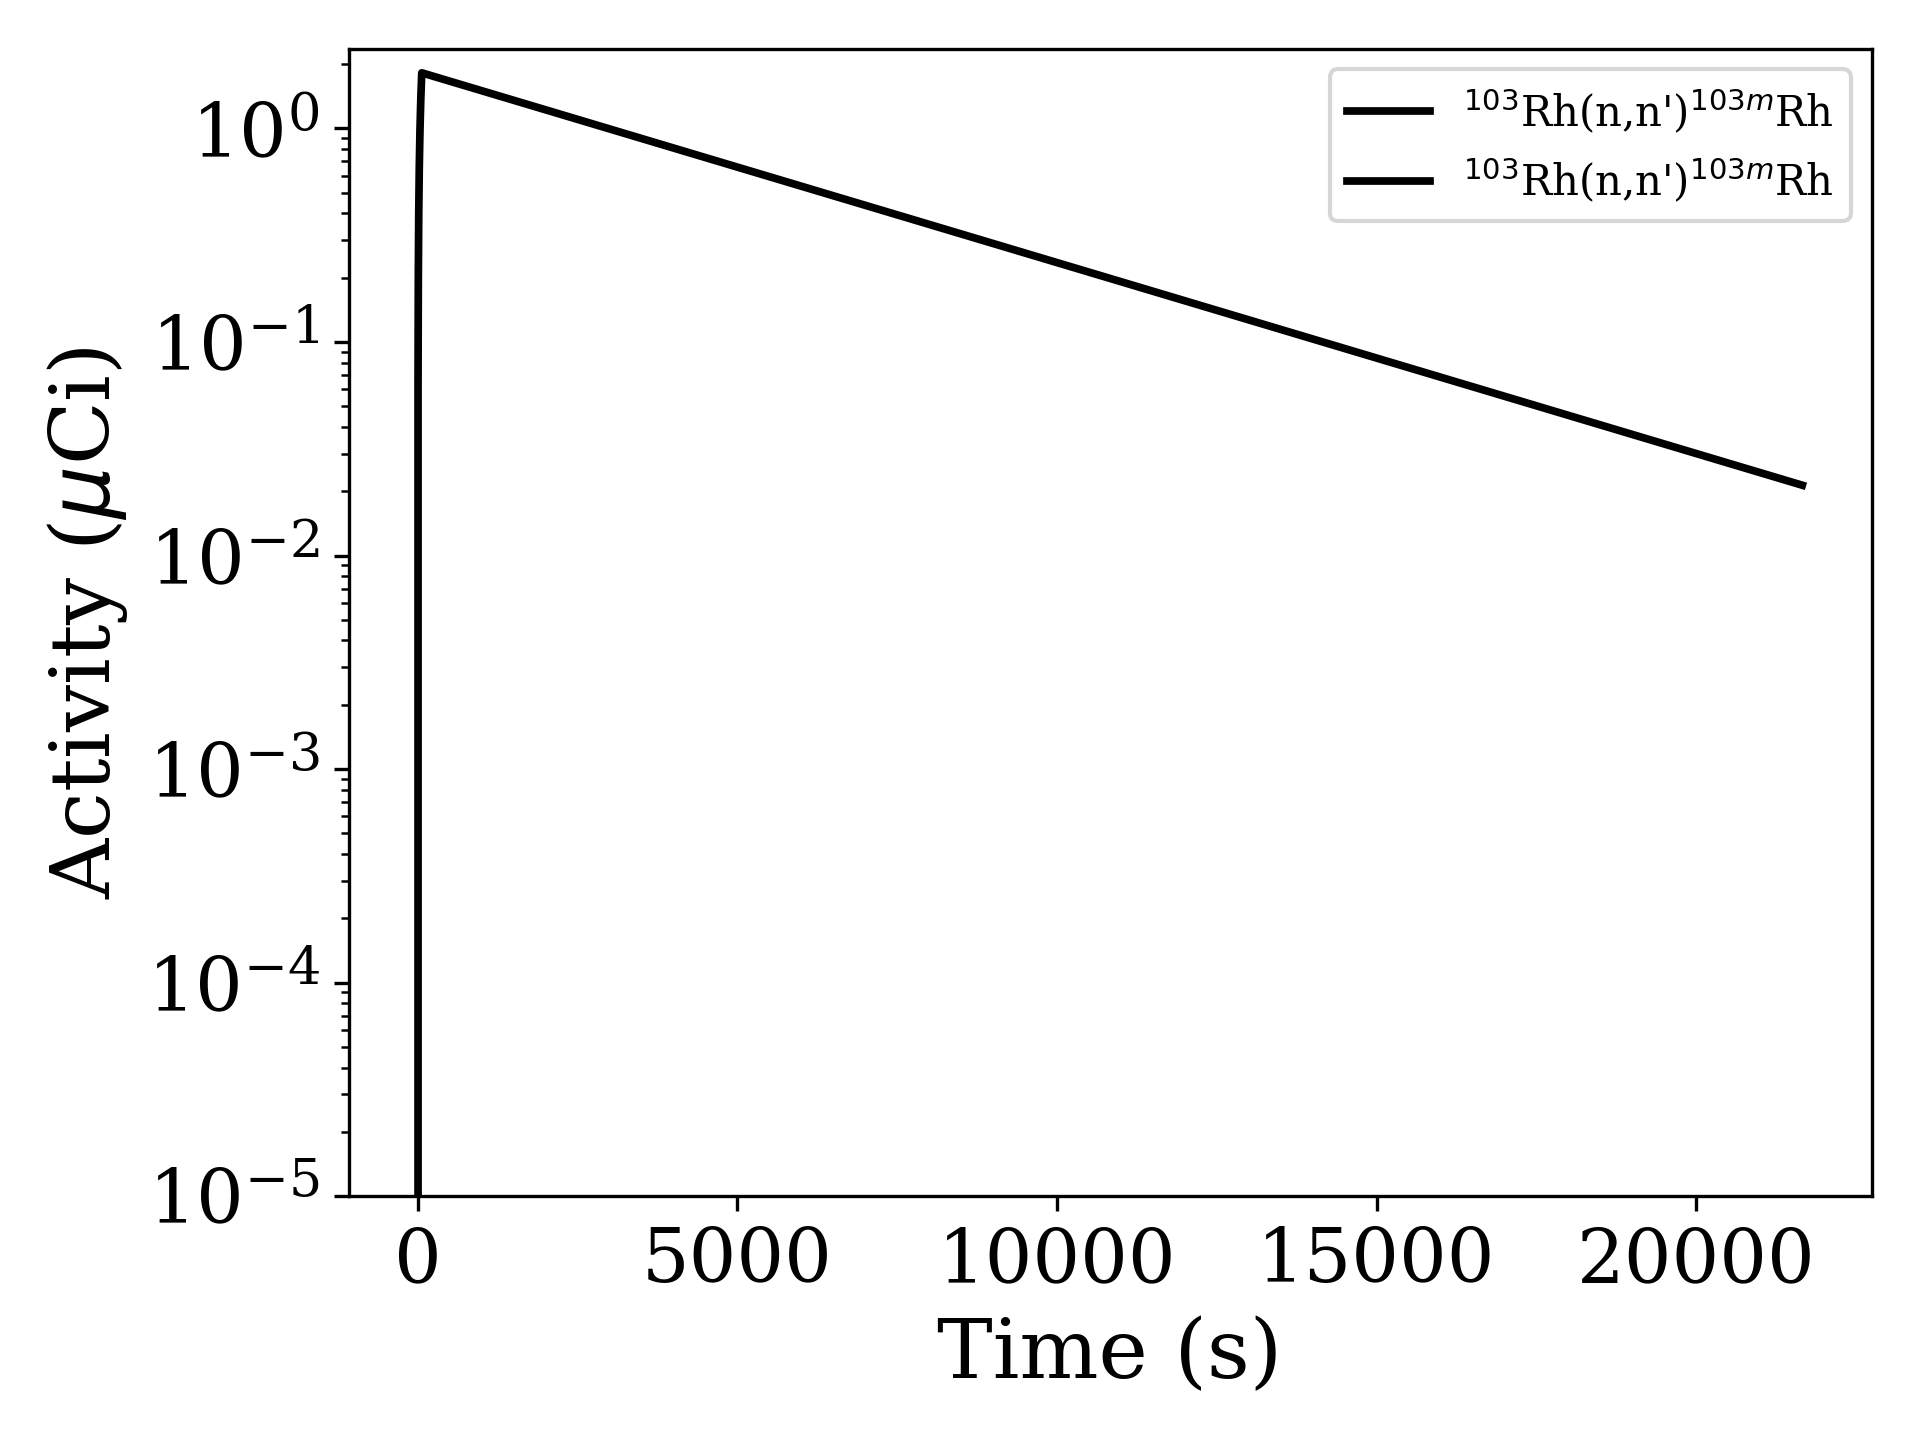
\includegraphics[width=.8\textwidth]{plot/Rh-103(n,n')Rh-103m_library1} 

  \caption{A subfigure}
  \label{fig:sub1}
\end{subfigure}%
\begin{subfigure}{.5\textwidth}
  \centering
     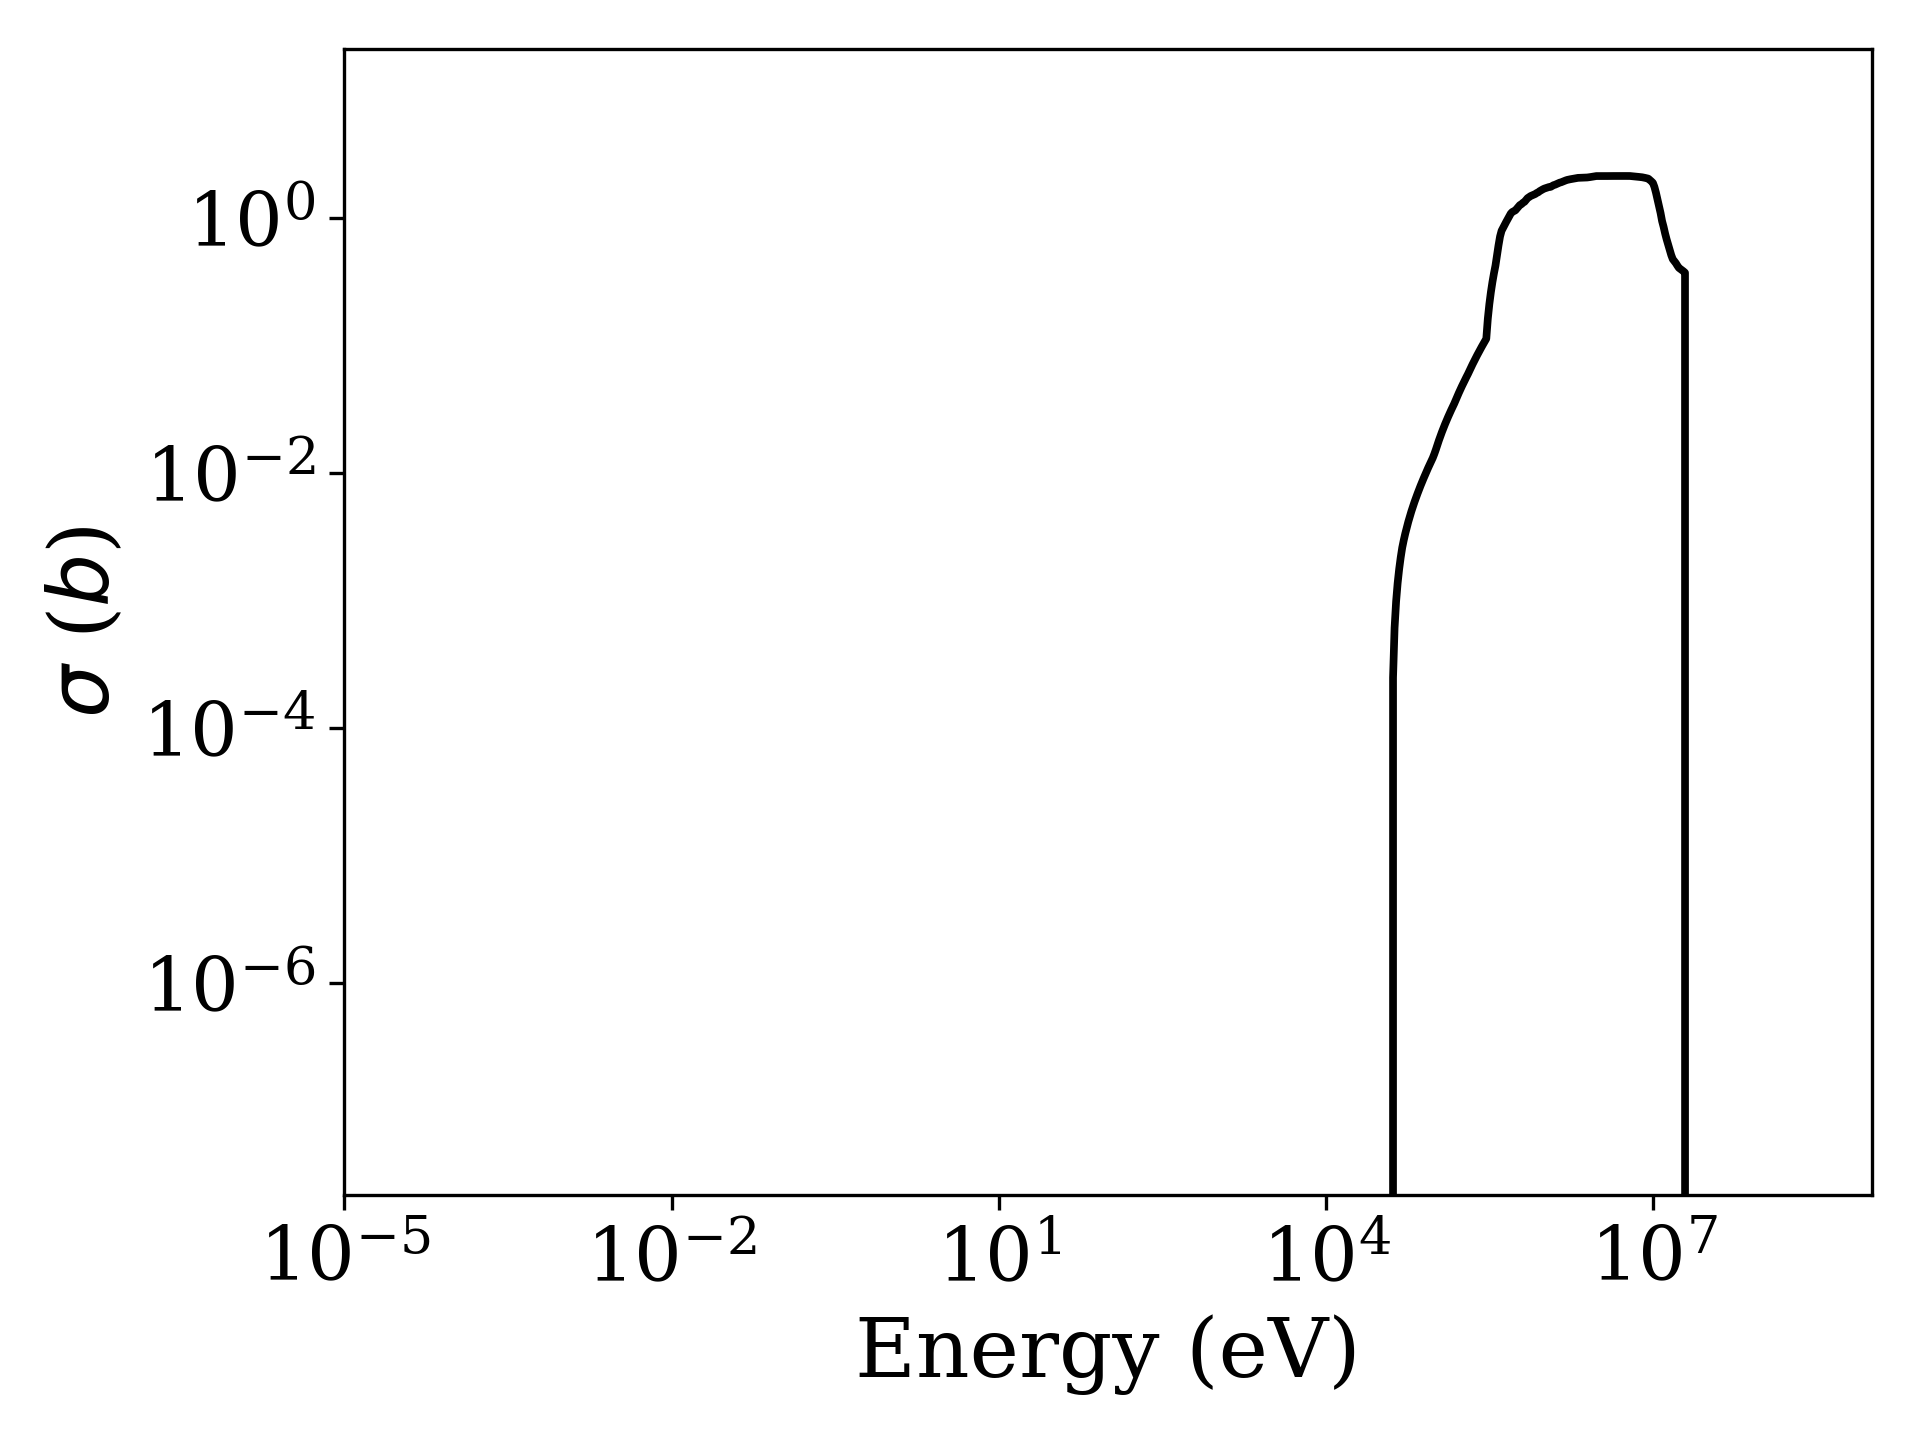
\includegraphics[width=.8\textwidth]{plot/Rh-103(n,n')Rh-103m} 

  \caption{A subfigure}
  \label{fig:sub2}
\end{subfigure}
\caption{A figure with two subfigures}
\label{fig:test}
\end{figure}

\begin{table*}[h]
\centering
\begin{tabular}{ |c|c|c|c|c|c|c| }
 \hline
 Reaction & T$_{1/2}$ & ROI (eV) & Important Gammas (keV) \\
 \hline 
 $^{103}$Rh(n,n')$^{103m}$Rh & 56.1 m & 4.91e+05, 5.21e+06 & 39.755(0.00068) \\ 
\hline
\end{tabular}
\end{table*}
